\documentclass[10pt,letterpaper]{article}
%\usepackage[utf8]{inputenc} % utf8 es usado por defecto en la mayoría de los casos
\usepackage[spanish]{babel}
\usepackage{csquotes} % Usar solo si spanish es seleccionado en babel
\usepackage{amsmath,amsfonts,amssymb,mathtools,bm} % Para funciones matemáticas especiales
\usepackage[%
    backend=biber, %bibtex8 o bibtex son antiguos y deben usarse solo por compatibilidad regresiva
	style=authoryear,
    natbib=true,
	doi=false,
	isbn=false,
	url=false,
	sorting=nyt,
	giveninits=true,% Abbreviates names
	uniquename=false,% Delete the initial in the reference. Compatible with firstinits/giveninits
	maxbibnames=15, % Max number of author per citation in the bibliography
	maxcitenames=2, % Max number of author per citation in the text
	dashed=false,   % false: Get full name twice in Bibliography
    ]{biblatex}
%\bibliography{bibfile} % for bibtex8
\addbibresource{bibfile.bib} % for biber

% Paquetes opcionales
\usepackage{graphicx,subfigure}
\usepackage{siunitx} 	% Unidades de medida según SI
\usepackage{booktabs}	% Para el toprule, midrule y bottomrule de las tablas
\usepackage{verbatim}

% Formato del borrador
\usepackage[font=small,labelfont=bf]{caption}
\usepackage[right=2cm,left=2.5cm,top=2.5cm,bottom=2.0cm,headsep=1cm,footskip=1.5cm]{geometry} % Page margins

% Headings
\title{Análisis carga--deflexión de una viga simplemente apoyada}
\author{Scarlette Vargas Guerrero\\
        {\footnotesize Departamento de Ingeniería en Obras Civiles, Universidad de Santiago de Chile}
}
%\date{28 de diciembre de 2018} % fecha de entrega
\date{\today}

% Figures path
\graphicspath{{figures/}} 

% Document information
\usepackage{hyperref}
\hypersetup{
	    pdfauthor = {Autores},
	    pdftitle = {Title},
	    pdfsubject = {Tema del trabajo},
	    pdfkeywords = {keyword 1, keyword 2,etc},
	    %draft,
	    %colorlinks,
        }


\begin{document}

% First pages
\maketitle

% Text body
\begin{abstract}
Se analizó una viga simplemente apoyada con una carga puntual aplicada en el centro de la luz, utilizando datos sintéticos entregados con fines docentes. El caso considera una sección rectangular de ancho \SI{0,2}{\meter} y altura \SI{0,4}{\meter}, una luz de \SI{4}{\meter} y un módulo de elasticidad de \SI{25}{\giga\pascal}. A partir de estos parámetros se realizó el cálculo del segundo momento de área y de la deflexión teórica mediante el modelo de Euler--Bernoulli para una carga puntual centrada. Posteriormente, se compararon las deflexiones teóricas con las deflexiones medidas para cargas entre \SI{0}{\kilo\newton} y \SI{40}{\kilo\newton}. La diferencia relativa máxima obtenida fue de \SI{4}{\percent}, correspondiente a la carga de \SI{5}{\kilo\newton}, mientras que para \SI{40}{\kilo\newton} la deflexión medida fue de \SI{2,05}{\milli\meter} frente a una deflexión teórica de \SI{2,00}{\milli\meter}. Los resultados muestran una concordancia cercana entre ambas series y una respuesta aproximadamente lineal. Finalmente, se realizaron verificaciones independientes del segundo momento de área y de valores puntuales de la deflexión teórica.
\end{abstract}


\section{Introducción}

La respuesta carga--deflexión de una viga simplemente apoyada permite comparar el comportamiento observado con una predicción basada en la teoría de Euler--Bernoulli. En este Hito 1 se estudia una viga con una carga puntual aplicada en el centro de la luz, utilizando datos sintéticos preparados exclusivamente con fines docentes.

El objetivo del análisis es construir un flujo reproducible que permita identificar los archivos de entrada, documentar las conversiones de unidades, calcular el segundo momento de área de la sección y obtener la deflexión teórica para cada nivel de carga. Posteriormente, los resultados teóricos se comparan con los datos de deflexión proporcionados.

La organización del trabajo mantiene separados los archivos originales, los cálculos, las figuras y la documentación, de modo que otra persona pueda rastrear el origen de los datos y reproducir el procedimiento empleado.


\section{Desarrollo}

El desarrollo se estructuró en cuatro etapas: identificación de los parámetros geométricos y mecánicos, conversión de unidades, cálculo de la respuesta teórica y comparación con los datos proporcionados. Los archivos originales corresponden a los datos de carga y deflexión, los parámetros geométricos y el módulo de elasticidad, además del esquema de la viga.

\subsection{Descripción del ensayo}

El sistema corresponde a una viga simplemente apoyada con una carga puntual aplicada en el centro de la luz. La longitud entre apoyos es \SI{4}{\meter}, mientras que la sección transversal es rectangular, con ancho \SI{0,2}{\meter} y altura \SI{0,4}{\meter}. El módulo de elasticidad entregado para el ejercicio es \SI{25}{\giga\pascal}.

El esquema de la configuración se muestra en la Fig.~\ref{fig:esquema_viga}. La carga se aplica en el centro de la luz, que corresponde al punto en el cual se registra la deflexión utilizada para la comparación.

\begin{figure}[hbtp]
\centering
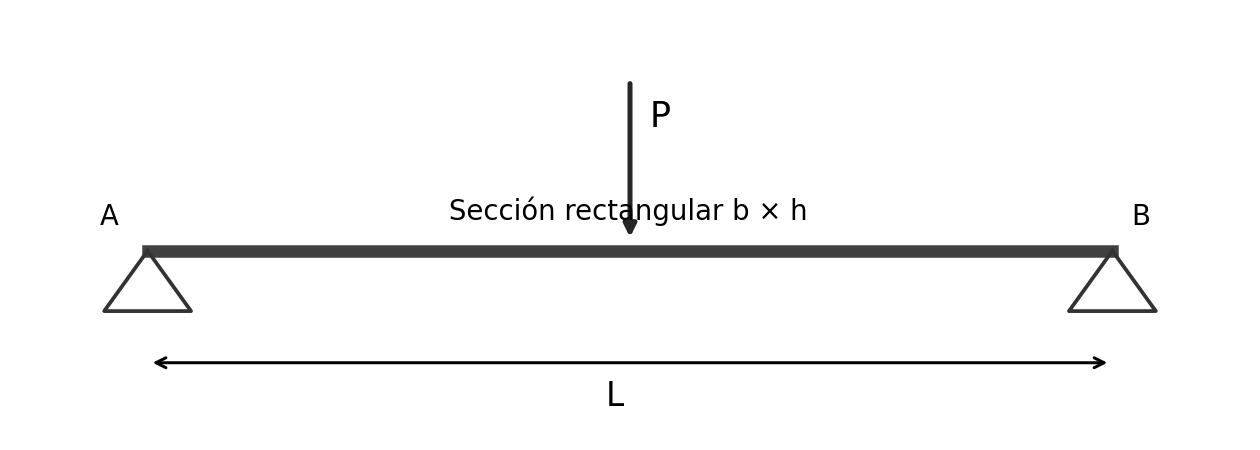
\includegraphics[width=0.78\textwidth]{figures/esquema_viga.png}
\caption{Viga simplemente apoyada con carga puntual centrada y sección rectangular.}
\label{fig:esquema_viga}
\end{figure}

Los datos de carga--deflexión fueron proporcionados en el archivo \verb|datos_viga.csv|. El archivo contiene nueve niveles de carga entre \SI{0}{\kilo\newton} y \SI{40}{\kilo\newton}, junto con la deflexión medida correspondiente. Estos datos son sintéticos y fueron preparados exclusivamente con fines docentes.


\subsection{Método de cálculo}

Para trabajar con unidades consistentes, los parámetros originales se transformaron al sistema compuesto por milímetros, newtons y megapascales. Las conversiones utilizadas fueron

\begin{equation}
L=\SI{4}{\meter}=\SI{4000}{\milli\meter},
\end{equation}

\begin{equation}
b=\SI{0,2}{\meter}=\SI{200}{\milli\meter},
\end{equation}

\begin{equation}
h=\SI{0,4}{\meter}=\SI{400}{\milli\meter},
\end{equation}

\begin{equation}
E=\SI{25}{\giga\pascal}=\SI{25000}{\mega\pascal}.
\end{equation}

Para una sección rectangular, el segundo momento de área respecto al eje neutro se calculó mediante

\begin{equation}
I=\frac{bh^3}{12}.
\end{equation}

Reemplazando los valores convertidos se obtiene

\begin{equation}
I=
\frac{(200)(400)^3}{12}
=
\SI{1,066666667e9}{\milli\meter^4}.
\end{equation}

La deflexión teórica en el centro de una viga simplemente apoyada sometida a una carga puntual centrada se calculó mediante \cite{Roylance2000}

\begin{equation}
\delta_{\mathrm{teo}}=
\frac{PL^3}{48EI}.
\end{equation}

Para aplicar esta expresión de manera consistente, las cargas del archivo de datos se transformaron de \si{\kilo\newton} a \si{\newton}. La deflexión obtenida mediante la expresión anterior se comparó con la deflexión medida para cada carga distinta de cero.

La diferencia absoluta se definió como

\begin{equation}
\Delta \delta =
\left|
\delta_{\mathrm{medida}}
-
\delta_{\mathrm{teo}}
\right|,
\end{equation}

mientras que la diferencia relativa se calculó mediante

\begin{equation}
e_r=
\frac{
\left|
\delta_{\mathrm{medida}}
-
\delta_{\mathrm{teo}}
\right|
}{
\delta_{\mathrm{teo}}
}
\,100.
\end{equation}

La carga nula se mantuvo como punto de referencia y no se utilizó para calcular la diferencia relativa, debido a que la deflexión teórica es igual a cero.


\subsection{Resultados y análisis}

Los resultados de la comparación entre la deflexión medida y la deflexión teórica se presentan en el Cuadro~\ref{table:deflexion}. La respuesta teórica aumenta linealmente con la carga, mientras que los datos proporcionados siguen una tendencia muy cercana.

\begin{table}[hbtp]
\caption{Comparación entre deflexión medida y deflexión teórica.}
\footnotesize
\centering
\begin{tabular}{cccc}
\toprule
\textit{Carga} &
\textit{Deflexión medida} &
\textit{Deflexión teórica} &
\textit{Error relativo} \\
\midrule
\SI{0}{\kilo\newton}  & \SI{0,00}{\milli\meter} & \SI{0,00}{\milli\meter} & -- \\
\SI{5}{\kilo\newton}  & \SI{0,26}{\milli\meter} & \SI{0,25}{\milli\meter} & \SI{4,00}{\percent} \\
\SI{10}{\kilo\newton} & \SI{0,50}{\milli\meter} & \SI{0,50}{\milli\meter} & \SI{0,00}{\percent} \\
\SI{15}{\kilo\newton} & \SI{0,76}{\milli\meter} & \SI{0,75}{\milli\meter} & \SI{1,33}{\percent} \\
\SI{20}{\kilo\newton} & \SI{1,01}{\milli\meter} & \SI{1,00}{\milli\meter} & \SI{1,00}{\percent} \\
\SI{25}{\kilo\newton} & \SI{1,28}{\milli\meter} & \SI{1,25}{\milli\meter} & \SI{2,40}{\percent} \\
\SI{30}{\kilo\newton} & \SI{1,54}{\milli\meter} & \SI{1,50}{\milli\meter} & \SI{2,67}{\percent} \\
\SI{35}{\kilo\newton} & \SI{1,77}{\milli\meter} & \SI{1,75}{\milli\meter} & \SI{1,14}{\percent} \\
\SI{40}{\kilo\newton} & \SI{2,05}{\milli\meter} & \SI{2,00}{\milli\meter} & \SI{2,50}{\percent} \\
\bottomrule
\end{tabular}
\label{table:deflexion}
\end{table}

La diferencia relativa máxima corresponde a la carga de \SI{5}{\kilo\newton}, con un valor de \SI{4,00}{\percent}. Para \SI{10}{\kilo\newton}, ambas deflexiones coinciden en \SI{0,50}{\milli\meter}. En el extremo superior de carga, a \SI{40}{\kilo\newton}, la diferencia absoluta es de \SI{0,05}{\milli\meter}, mientras que el error relativo es de \SI{2,50}{\percent}.

La comparación completa se representa en la Fig.~\ref{fig:carga_deflexion}. Ambas series presentan una tendencia prácticamente lineal y permanecen próximas en todo el rango de carga analizado.

\begin{figure}[hbtp]
\centering
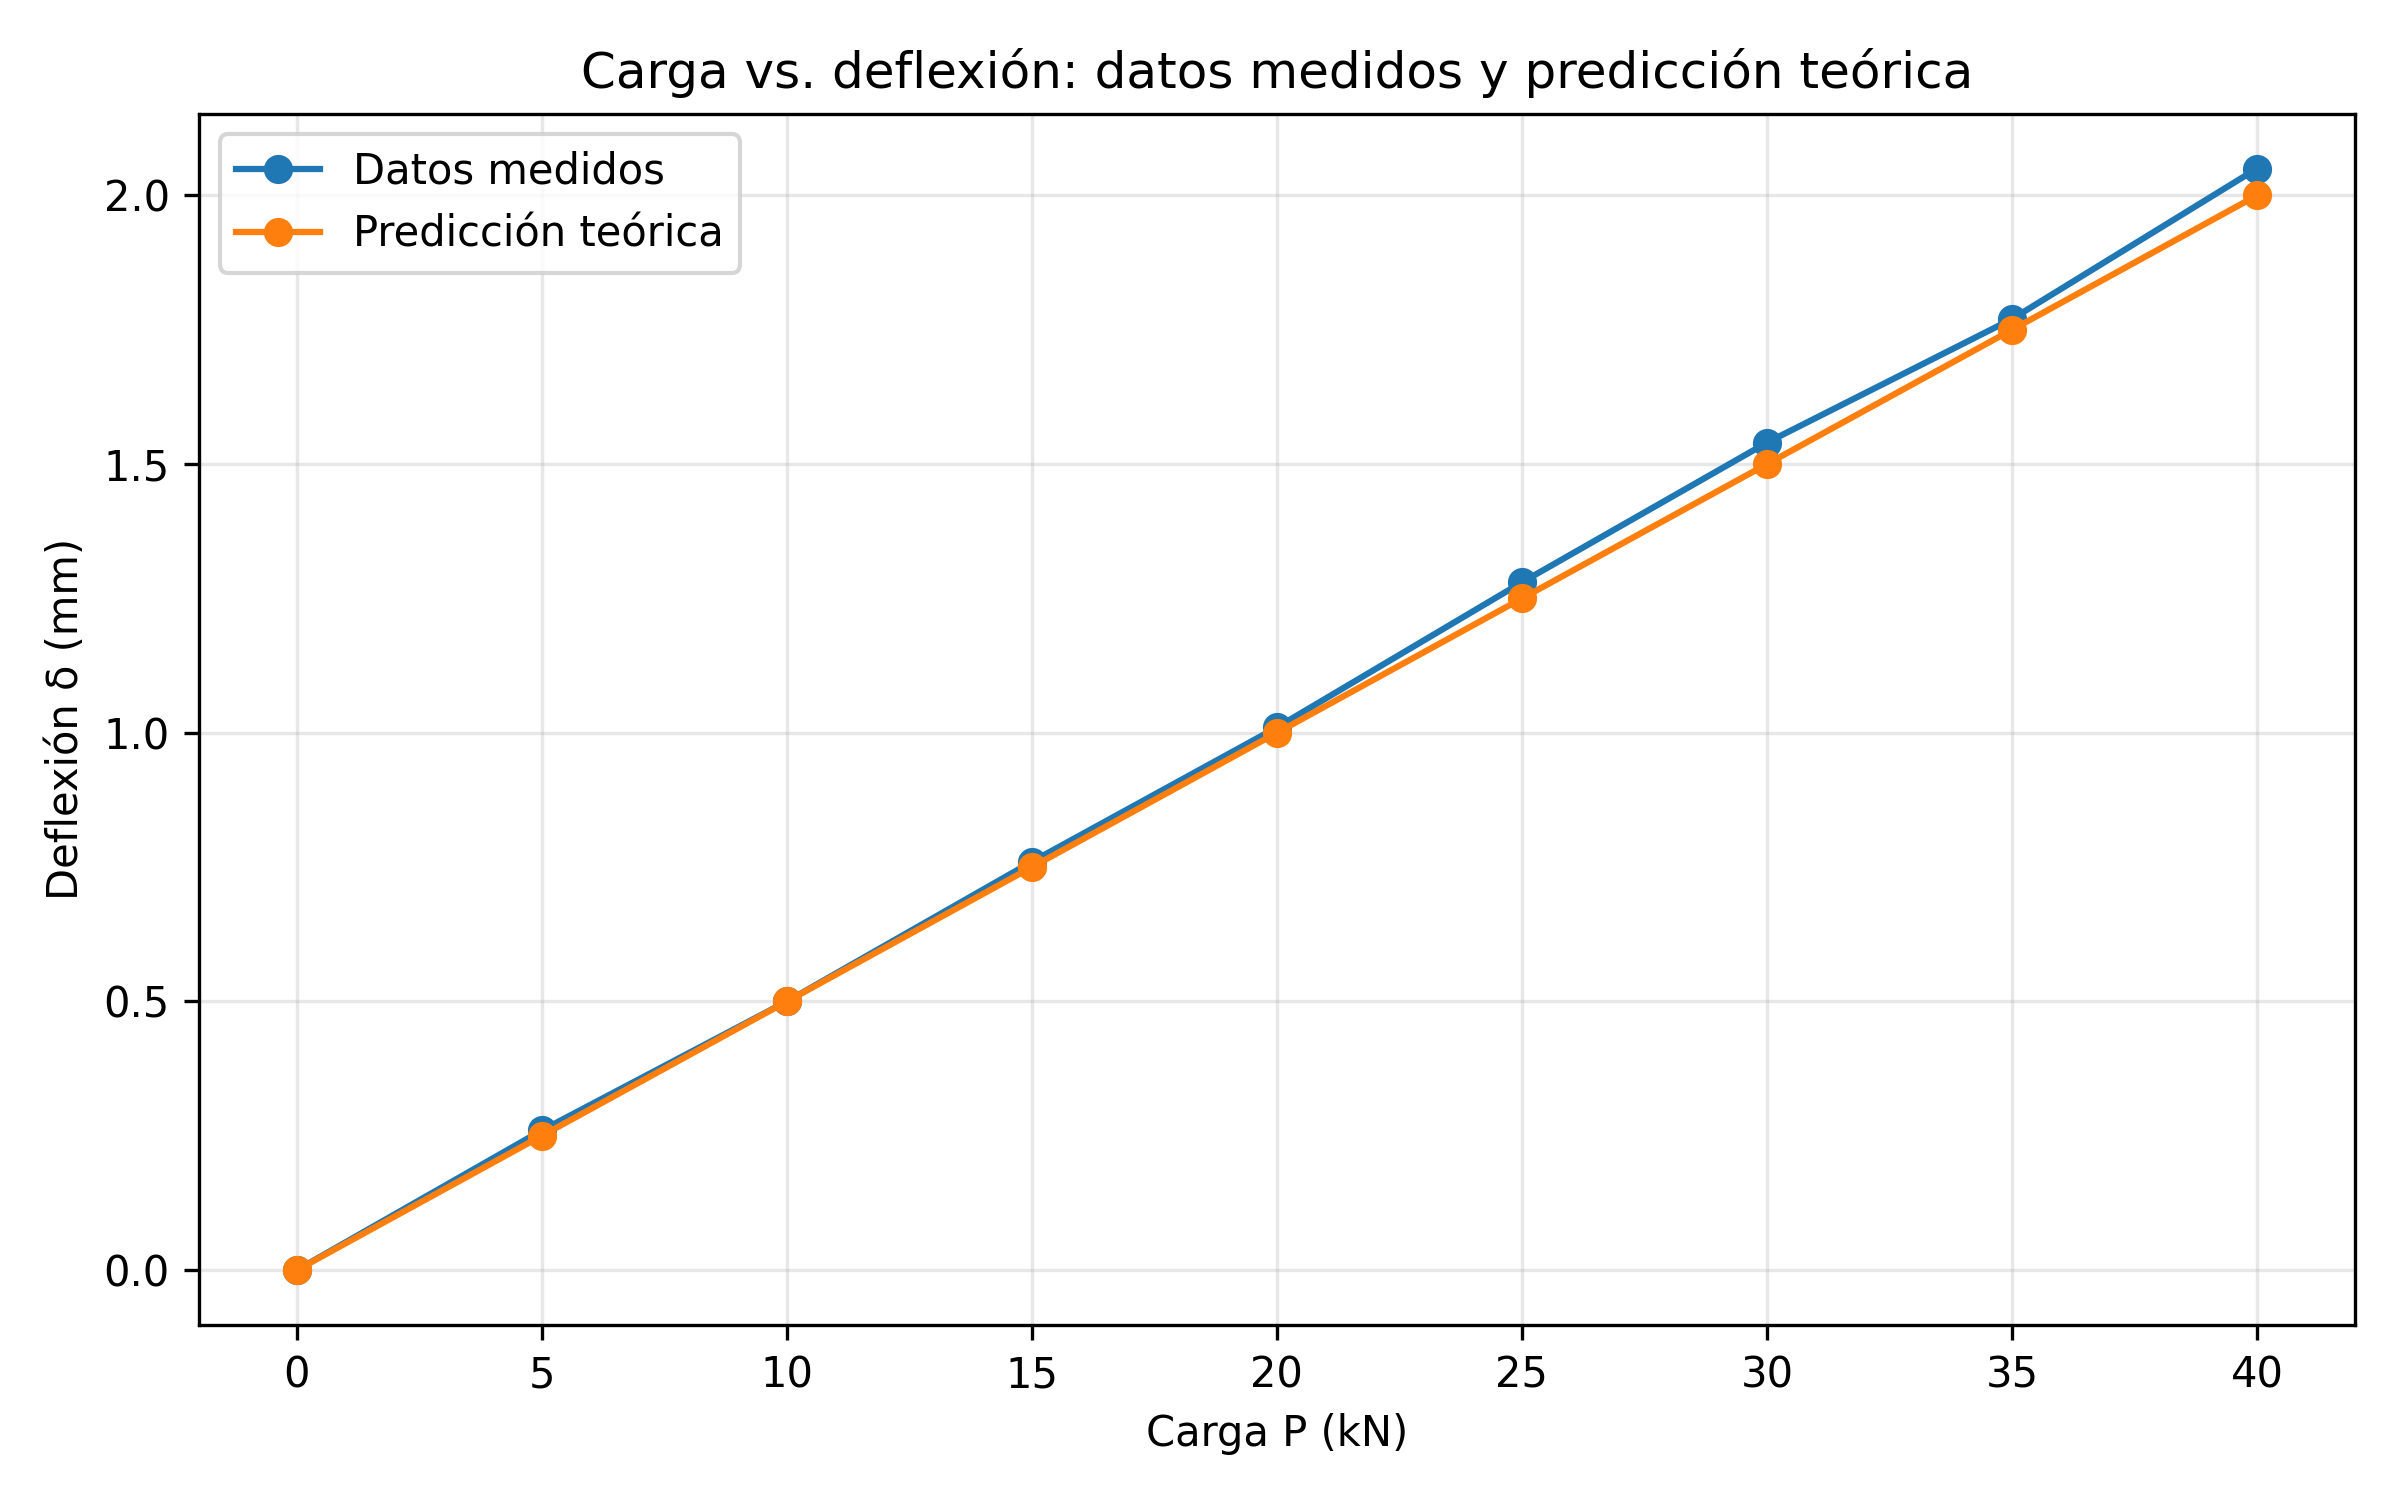
\includegraphics[width=0.88\textwidth]{figures/carga_deflexion_hito1.png}
\caption{Comparación entre los datos de carga--deflexión medidos y la predicción teórica de Euler--Bernoulli.}
\label{fig:carga_deflexion}
\end{figure}

Como verificación adicional, se comprobó de manera independiente el cálculo del segundo momento de área y dos valores de la deflexión teórica. El resultado calculado de \(I\) fue \SI{1,066666667e9}{\milli\meter^4}, coincidente con el valor obtenido mediante la expresión geométrica de la sección. Asimismo, para cargas de \SI{20}{\kilo\newton} y \SI{40}{\kilo\newton}, las deflexiones teóricas calculadas fueron respectivamente \SI{1,00}{\milli\meter} y \SI{2,00}{\milli\meter}. Estas comprobaciones independientes permiten verificar la consistencia de las fórmulas y de las unidades antes de utilizar los resultados en la figura.

Los resultados deben interpretarse considerando que los datos son sintéticos y fueron generados exclusivamente con fines docentes. Por esta razón, la comparación no representa una validación experimental de la teoría, sino una verificación de la coherencia entre los datos proporcionados y el modelo de cálculo solicitado.


\section{Conclusiones y perspectivas}

El análisis permitió construir un flujo de cálculo reproducible para una viga simplemente apoyada con carga puntual centrada. A partir de la geometría entregada se obtuvo un segundo momento de área de \SI{1,066666667e9}{\milli\meter^4}, y se calcularon las deflexiones teóricas mediante la expresión de Euler--Bernoulli.

La comparación mostró una concordancia cercana entre las deflexiones medidas y teóricas. El error relativo máximo fue de \SI{4,00}{\percent}, mientras que a \SI{40}{\kilo\newton} la diferencia fue de solo \SI{0,05}{\milli\meter}. La tendencia prácticamente lineal de ambas series es consistente con el modelo elástico empleado para el análisis.

Las verificaciones adicionales del segundo momento de área y de valores puntuales de la deflexión teórica confirmaron la consistencia de los cálculos realizados. Como principal limitación, se debe considerar que los datos utilizados son sintéticos y, por lo tanto, no permiten evaluar la correspondencia con un ensayo experimental real.

Como perspectiva de mejora, el mismo flujo podría ampliarse incorporando nuevas series de datos y automatizando la generación de tablas y figuras a partir de los archivos de entrada, manteniendo la misma estructura reproducible del repositorio.

% References
\renewcommand*{\bibfont}{\footnotesize}
\printbibliography%[sorting=nyt]

\end{document}